\section{ 新しいドア~冬のひまわり~}

\parpic[r]{
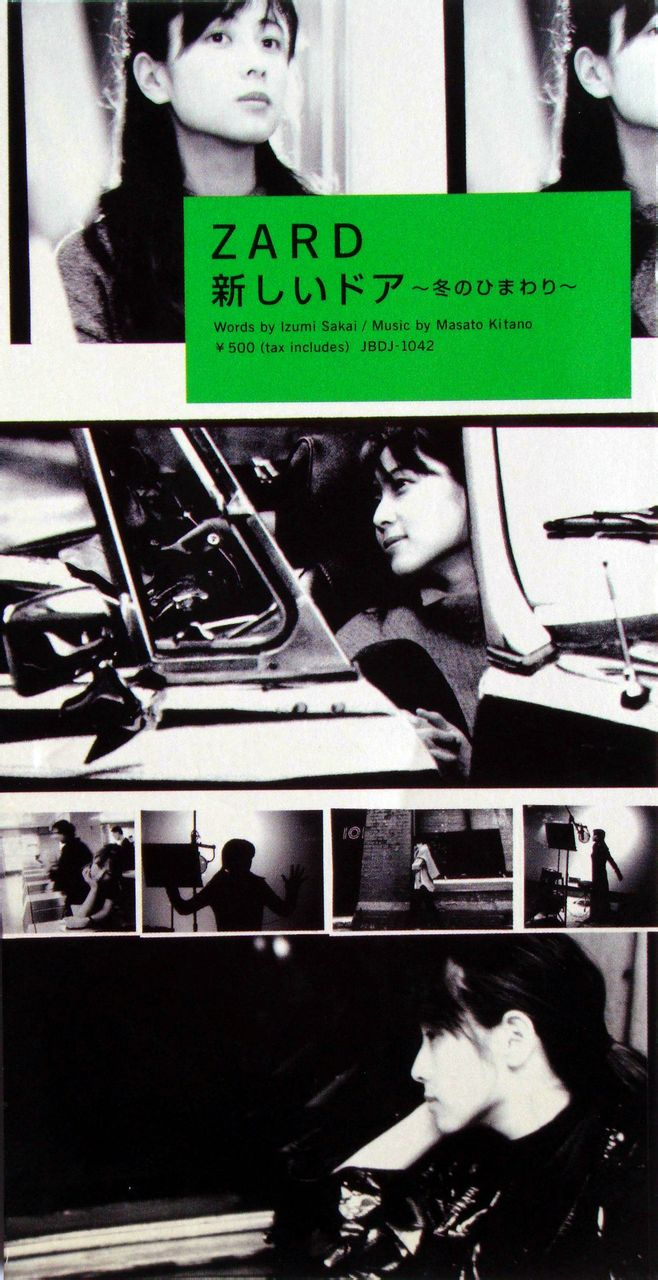
\includegraphics[width=0.3\textwidth]{S26.jpg}}

\large{

\ruby{通}{とお}り\ruby{雨}{あめ}の\ruby{中}{なか}で \ruby{抱}{だ}きしめた\ruby{君}{きみ}の\ruby{体温}{ぬくもり}

まだ この\ruby{胸}{むね}に \ruby{今}{いま}も \ruby{残}{のこ}っているよ
\\

\ruby{波}{なみ}に \ruby{揺}{ゆ}られながら

\ruby{泣}{な}いているだけの\ruby{夜}{よる}にサ·ヨ·ナ·ラ

\ruby{口笛}{くちぶえ}\ruby{吹}{ふ}いた あの\ruby{帰}{かえ}り\ruby{道}{みち}

ずっと \ruby{夕}{ゆ}\ruby{焼}{や}け \ruby{追}{お}いかけた
\\

はるかな\ruby{未来}{みらい}へと \ruby{新}{あたら}しい\ruby{ドア}{Door}を\ruby{開}{あ}け

\ruby{動}{うご}き\ruby{始}{はじ}めた \ruby{直感}{ちょっかん}が\ruby{行}{い}く\ruby{道}{みち}を\ruby{決}{き}める

あの\ruby{冬}{ふゆ}の\ruby{向日葵}{ひまわり}

まだひとりでやれそうだよ

\ruby{愛}{あい}する\ruby{人}{ひと}よ \ruby{今}{いま}どこで\ruby{眠}{ねむ}っていますか?

sweet pain \ruby{永遠}{えいえん}にとり\ruby{戻}{もど}せない あの\ruby{季節}{きせつ}
\\

\ruby{外}{そと}はこんなに \ruby{晴}{は}れているのに

\ruby{君}{きみ}の リンカクは ぼやけたまま

\ruby{無邪気}{むじゃき}に\ruby{笑}{わら}いあう あの\ruby{空}{そら}は\ruby{夢}{ゆめ}の\ruby{中}{なか}
\\

あの\ruby{時}{とき} \ruby{見}{み}えなかった\ruby{事}{こと}が

\ruby{今}{いま} \ruby{少}{すこ}しづつ わかりはじめているよ

スゴイケンカして \ruby{泣}{な}き\ruby{出}{だ}して\ruby{一人}{ひとり}

\ruby{先}{さき}に\ruby{帰}{かえ}った あの\ruby{渚}{なぎさ}
\\

\ruby{光}{ひか}る\ruby{夏}{なつ}に\ruby{生}{う}まれた \ruby{新}{あたら}しい\ruby{風}{かぜ}を\ruby{受}{う}け

まぶしい\ruby{空}{そら}を いくつも\ruby{超}{こ}えてゆきたい

\ruby{名前}{なまえ}なんか \ruby{知}{し}らなくても

\ruby{軽}{かる}い\ruby{ジョーク}{Joke}で\ruby{笑}{わら}えたね

あの\ruby{仲間達}{なかまたち} また\ruby{一緒}{いっしょ}に\ruby{行}{い}こうよ

I remember sweet memories

おかしいのに \ruby{何故}{なぜ}か\ruby{涙}{なみだ}が\ruby{出}{で}たよ
\\

はるかな\ruby{未来}{みらい}へと \ruby{新}{あたら}しい\ruby{ドア}{Door}を\ruby{開}{あ}け

\ruby{動}{うご}き\ruby{始}{はじ}めた \ruby{直感}{ちょっかん}が\ruby{行}{い}く\ruby{道}{みち}を\ruby{決}{き}める

あの\ruby{冬}{ふゆ}の\ruby{向日葵}{ひまわり}

まだひとりでやれそうだよ

\ruby{愛}{あい}する\ruby{人}{ひと}よ \ruby{今}{いま}どこで\ruby{眠}{ねむ}っていますか?

sweet pain \ruby{永遠}{えいえん}にとり\ruby{戻}{もど}せない あの\ruby{季節}{きせつ}
\\

sweet pain...
\\

\ruby{通}{とお}り\ruby{雨}{あめ}の\ruby{中}{なか}で \ruby{抱}{だ}きしめた\ruby{君}{きみ}の\ruby{体温}{ぬくもり}

まだこの\ruby{胸}{むね}に \ruby{今}{いま}も \ruby{残}{のこ}っているよ

}